\subsection{Developing the Loss Function}

Most of the time was spent developing the multi-part loss function \cite[Eq.3]{YOLO}, and this was a daunting task.
The formula given in the paper is deceptively simple and even after scouring many online implementations, it seems like everyone has slightly different ways of approaching this loss function.
Truth be told, we don't believe that our implementation ended up as the author of \cite{YOLO} intended, but it worked fairly well and so we went with it.

We approached this task by first trying to learn very simple bounding boxes, in particular, we learn randomly generated rectangles as in \Cref{Figure:Face-Detection:loss-function:rectangles-example}.

\begin{figure}[htbp]
    \centering
    \begin{subfigure}{0.32\textwidth}
        \centering
        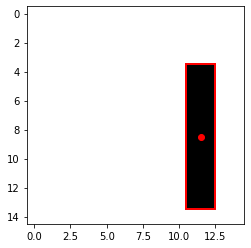
\includegraphics[width=0.95\textwidth]{images/faceDetec/loss-function/rectangle-example.png}
    \end{subfigure}
    \hfill
    \begin{subfigure}{0.32\textwidth}
        \centering
        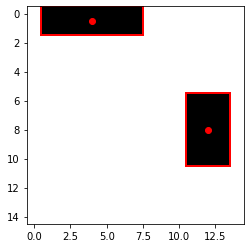
\includegraphics[width=0.95\textwidth]{images/faceDetec/loss-function/rectangle-example-2.png}
    \end{subfigure}
    \hfill
    \begin{subfigure}{0.32\textwidth}
        \centering
        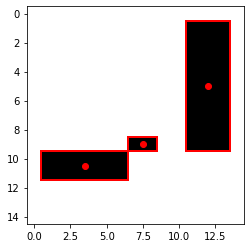
\includegraphics[width=0.95\textwidth]{images/faceDetec/loss-function/rectangle-example-3.png}
    \end{subfigure}
    \caption{Our first task is to learn randomly generated images containing 1, 2 or 3 rectangles. The red outline is the bounding box and the dot is the center of the box.}
    \label{Figure:Face-Detection:loss-function:rectangles-example}
\end{figure}

To that end, using the simple model described in \Cref{Table:Face-Detection:rectangles-model} to attain $\sim75\%$ accuracy on 100 randomly generated rectangle plots.

\begin{table}[htbp]
    \centering
    \begin{tabular}{c|c|c|c}
        Type            & Filters  & Size         & Output            \\
        \hline
        Input           &          &              & $15 \times 15$    \\
        Convolutional   & 128      & $5 \times 5$ & $15 \times 15$    \\
        Convolutional   & 128      & $5 \times 5$ & $15 \times 15$    \\
        Convolutional   & 128      & $5 \times 5$ & $15 \times 15$    \\
        Fully Connected &          & $90$         &                   \\
    \end{tabular}
    \caption{
        A simple model to learn the randomly generated rectangles (\Cref{Figure:Face-Detection:loss-function:rectangles-example}).
        Each convolutional layer is followed by a Batch Normalization layer and the activation function we chose is Leaky ReLU with a gradient of 0.1.
    }
    \label{Table:Face-Detection:rectangles-model}
\end{table}

We present a couple of the predictions in \Cref{Figure:Face-Detection:loss-function:rectangles-predictions} for completeness.
The code for the loss function can be found in the notebook: \href{https://github.com/nicholaspun/IZ-Net/blob/master/notebooks/ObjectDetectionTest.ipynb}{\inlinecode{ObjectDetectionTest.ipynb}}

\begin{figure}[htbp]
    \centering
    \begin{subfigure}{0.32\textwidth}
        \centering
        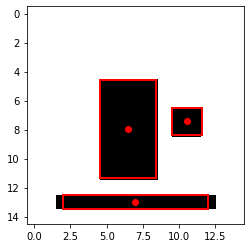
\includegraphics[width=0.95\textwidth]{images/faceDetec/loss-function/rectangle-prediction-1.png}
    \end{subfigure}
    \hfill
    \begin{subfigure}{0.32\textwidth}
        \centering
        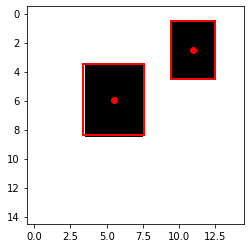
\includegraphics[width=0.95\textwidth]{images/faceDetec/loss-function/rectangle-prediction-2.png}
    \end{subfigure}
    \hfill
    \begin{subfigure}{0.32\textwidth}
        \centering
        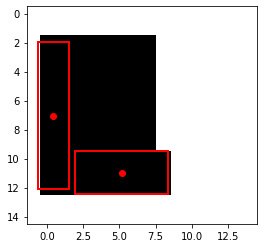
\includegraphics[width=0.95\textwidth]{images/faceDetec/loss-function/rectangle-prediction-3.png}
    \end{subfigure}
    \caption{
        Sample predictions given by our simple model in \Cref{Table:Face-Detection:rectangles-model}.
        Notice the slight inaccuracies in the bounding boxes as well as the bounding box that was completely missed in the rightmost image.
        As a side note, most of the erroneous predictions came from plots with overlapping rectangles, which actually may have been throwing off the model.
    }
    \label{Figure:Face-Detection:loss-function:rectangles-predictions}
\end{figure}